% Options for packages loaded elsewhere
\PassOptionsToPackage{unicode}{hyperref}
\PassOptionsToPackage{hyphens}{url}
%
\documentclass[
  12pt,
  ignorenonframetext,
  aspectratio=169,
]{beamer}
\usepackage{pgfpages}
\setbeamertemplate{caption}[numbered]
\setbeamertemplate{caption label separator}{: }
\setbeamercolor{caption name}{fg=normal text.fg}
\beamertemplatenavigationsymbolsempty
% Prevent slide breaks in the middle of a paragraph
\widowpenalties 1 10000
\raggedbottom

\usepackage{amsmath,amssymb}
\usepackage{iftex}
\ifPDFTeX
  \usepackage[T1]{fontenc}
  \usepackage[utf8]{inputenc}
  \usepackage{textcomp} % provide euro and other symbols
\else % if luatex or xetex
  \usepackage{unicode-math}
  \defaultfontfeatures{Scale=MatchLowercase}
  \defaultfontfeatures[\rmfamily]{Ligatures=TeX,Scale=1}
\fi
\usepackage{lmodern}
\ifPDFTeX\else  
    % xetex/luatex font selection
\fi
% Use upquote if available, for straight quotes in verbatim environments
\IfFileExists{upquote.sty}{\usepackage{upquote}}{}
\IfFileExists{microtype.sty}{% use microtype if available
  \usepackage[]{microtype}
  \UseMicrotypeSet[protrusion]{basicmath} % disable protrusion for tt fonts
}{}
\makeatletter
\@ifundefined{KOMAClassName}{% if non-KOMA class
  \IfFileExists{parskip.sty}{%
    \usepackage{parskip}
  }{% else
    \setlength{\parindent}{0pt}
    \setlength{\parskip}{6pt plus 2pt minus 1pt}}
}{% if KOMA class
  \KOMAoptions{parskip=half}}
\makeatother
\usepackage{xcolor}
\newif\ifbibliography
\setlength{\emergencystretch}{3em} % prevent overfull lines
\setcounter{secnumdepth}{-\maxdimen} % remove section numbering


\providecommand{\tightlist}{%
  \setlength{\itemsep}{0pt}\setlength{\parskip}{0pt}}\usepackage{longtable,booktabs,array}
\usepackage{calc} % for calculating minipage widths
\usepackage{caption}
% Make caption package work with longtable
\makeatletter
\def\fnum@table{\tablename~\thetable}
\makeatother
\usepackage{graphicx}
\makeatletter
\def\maxwidth{\ifdim\Gin@nat@width>\linewidth\linewidth\else\Gin@nat@width\fi}
\def\maxheight{\ifdim\Gin@nat@height>\textheight\textheight\else\Gin@nat@height\fi}
\makeatother
% Scale images if necessary, so that they will not overflow the page
% margins by default, and it is still possible to overwrite the defaults
% using explicit options in \includegraphics[width, height, ...]{}
\setkeys{Gin}{width=\maxwidth,height=\maxheight,keepaspectratio}
% Set default figure placement to htbp
\makeatletter
\def\fps@figure{htbp}
\makeatother

\usepackage{booktabs}
\usepackage{longtable}
\usepackage{array}
\usepackage{multirow}
\usepackage{wrapfig}
\usepackage{float}
\usepackage{colortbl}
\usepackage{pdflscape}
\usepackage{tabu}
\usepackage{threeparttable}
\usepackage{threeparttablex}
\usepackage[normalem]{ulem}
\usepackage{makecell}
\usepackage{xcolor}
\makeatletter
\@ifpackageloaded{tcolorbox}{}{\usepackage[skins,breakable]{tcolorbox}}
\@ifpackageloaded{fontawesome5}{}{\usepackage{fontawesome5}}
\definecolor{quarto-callout-color}{HTML}{909090}
\definecolor{quarto-callout-note-color}{HTML}{0758E5}
\definecolor{quarto-callout-important-color}{HTML}{CC1914}
\definecolor{quarto-callout-warning-color}{HTML}{EB9113}
\definecolor{quarto-callout-tip-color}{HTML}{00A047}
\definecolor{quarto-callout-caution-color}{HTML}{FC5300}
\definecolor{quarto-callout-color-frame}{HTML}{acacac}
\definecolor{quarto-callout-note-color-frame}{HTML}{4582ec}
\definecolor{quarto-callout-important-color-frame}{HTML}{d9534f}
\definecolor{quarto-callout-warning-color-frame}{HTML}{f0ad4e}
\definecolor{quarto-callout-tip-color-frame}{HTML}{02b875}
\definecolor{quarto-callout-caution-color-frame}{HTML}{fd7e14}
\makeatother
\makeatletter
\@ifpackageloaded{caption}{}{\usepackage{caption}}
\AtBeginDocument{%
\ifdefined\contentsname
  \renewcommand*\contentsname{Table of contents}
\else
  \newcommand\contentsname{Table of contents}
\fi
\ifdefined\listfigurename
  \renewcommand*\listfigurename{List of Figures}
\else
  \newcommand\listfigurename{List of Figures}
\fi
\ifdefined\listtablename
  \renewcommand*\listtablename{List of Tables}
\else
  \newcommand\listtablename{List of Tables}
\fi
\ifdefined\figurename
  \renewcommand*\figurename{Figure}
\else
  \newcommand\figurename{Figure}
\fi
\ifdefined\tablename
  \renewcommand*\tablename{Table}
\else
  \newcommand\tablename{Table}
\fi
}
\@ifpackageloaded{float}{}{\usepackage{float}}
\floatstyle{ruled}
\@ifundefined{c@chapter}{\newfloat{codelisting}{h}{lop}}{\newfloat{codelisting}{h}{lop}[chapter]}
\floatname{codelisting}{Listing}
\newcommand*\listoflistings{\listof{codelisting}{List of Listings}}
\makeatother
\makeatletter
\makeatother
\makeatletter
\@ifpackageloaded{caption}{}{\usepackage{caption}}
\@ifpackageloaded{subcaption}{}{\usepackage{subcaption}}
\makeatother

\ifLuaTeX
  \usepackage{selnolig}  % disable illegal ligatures
\fi
\usepackage{bookmark}

\IfFileExists{xurl.sty}{\usepackage{xurl}}{} % add URL line breaks if available
\urlstyle{same} % disable monospaced font for URLs
\hypersetup{
  pdftitle={Uncertainty Estimation for High-dimensional Nonparametric Forecasting},
  pdfauthor={Nuwani Palihawadana},
  hidelinks,
  pdfcreator={LaTeX via pandoc}}

\usetheme{Monash}


% Monash title page
% Modified by moving title and adding collaborators
\setbeamerfont{title}{series=\bfseries,parent=structure,size=\fontsize{20}{28}}
\setbeamertemplate{title page}
{\placefig{-0.01}{-0.01}{width=1.01\paperwidth,height=1.01\paperheight}{bg-13.png}
\begin{textblock}{10.2}(1,1)\usebeamerfont{title}
{\color{white}\raggedright\par\inserttitle}
\end{textblock}
\begin{textblock}{8.7}(1,5.3)
{\color{white}\raggedright{\insertauthor}\mbox{}\\[0.2cm]}
\end{textblock}
\begin{textblock}{10.8}(1,6.6)
{\color{white}\raggedright{\textbf{Joint work with :} Rob Hyndman, Xiaoqian Wang}\mbox{}\\[0.2cm]
\insertdate}
\end{textblock}}


% Find images
\graphicspath{{_extensions/presentation/_images/background/}{_extensions/quarto-monash/presentation/_images/background/}{figs/}{figures/}{images/}{img/}}
\title{Uncertainty Estimation for High-dimensional Nonparametric
Forecasting}
\author{Nuwani Palihawadana}
\date{1 July 2025}
\titlegraphic{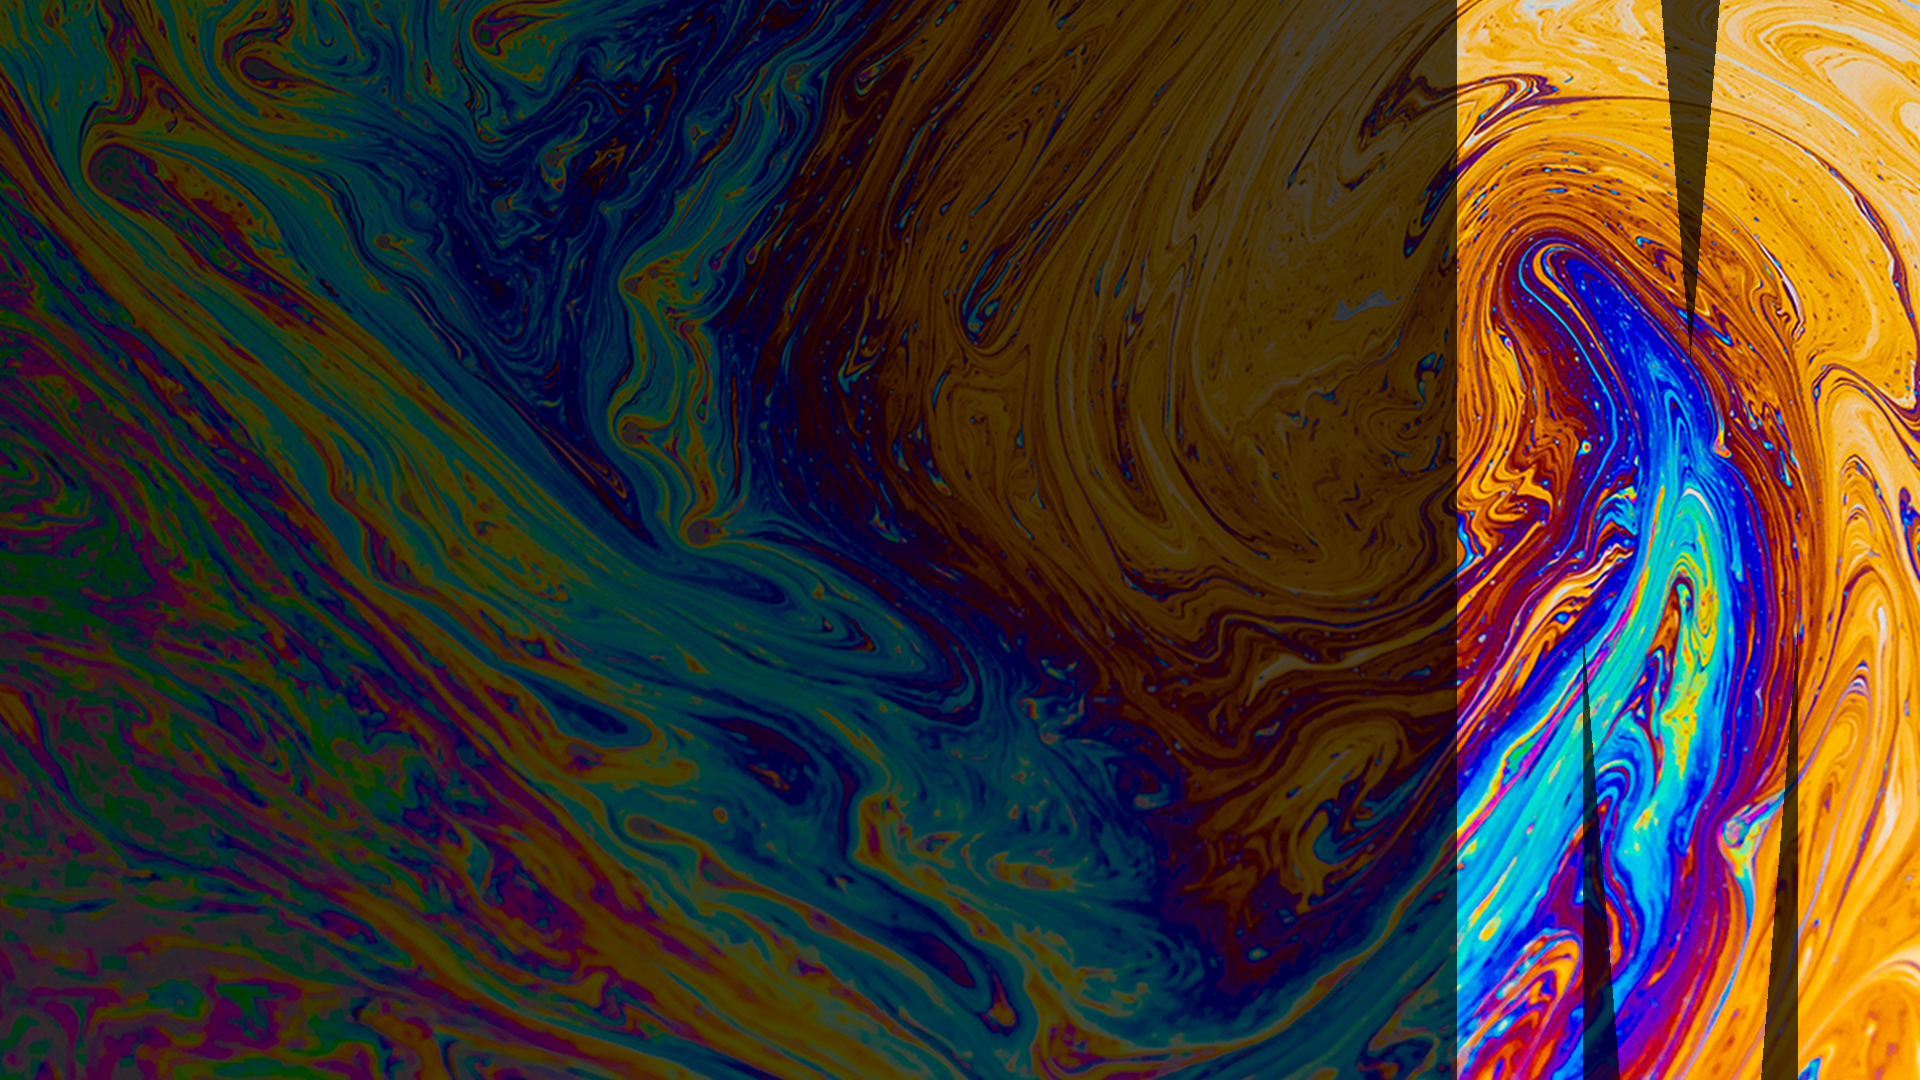
\includegraphics{bg-13.png}}

\begin{document}
\frame{\titlepage}


\begin{frame}{Nonparametric forecasting}
\phantomsection\label{nonparametric-forecasting}
\end{frame}

\begin{frame}{Sparse multiple index (SMI) model}
\phantomsection\label{sparse-multiple-index-smi-model}
\end{frame}

\begin{frame}{Benchmarks}
\phantomsection\label{benchmarks}
\end{frame}

\begin{frame}{Forecast uncertainty}
\phantomsection\label{forecast-uncertainty}
\begin{itemize}
  \item Uncertainty of a forecast \alert{${\rightarrow}$ Prediction Interval (PI)}
  \pause
  \item Theoretical $100(1 - \alpha)\%$ prediction interval:
$$
  \hat{y}_{t+h|t} \pm z_{\alpha/2} \times \hat{\sigma}_{h},
$$
where
  \begin{itemize}
    \item \small \color{black} $y$ -- \color{violet} time series $y_{1}, \dots, y_{T}$
    \item \small \color{black} $\hat{y}_{t+h|t}$ -- \color{violet} $h$-step-ahead point forecast for $y_{t+h}$ given observations up to $t$
    \item \small \color{black} $z_{\alpha/2}$ -- \color{violet} $\alpha/2$ quantile of standard normal distribution
    \item \small \color{black} $\hat{\sigma}_{h}$ -- \color{violet} estimate of std. deviation of $h$-step forecast distribution
  \end{itemize}
  \pause
  \item Main issue:
  \begin{itemize}
    \item \small \color{blue} Difficult to analytically calculate $h$-step forecast variances for $h > 1$
  \end{itemize}
\end{itemize}
\end{frame}

\begin{frame}{Block bootstrap}
\phantomsection\label{block-bootstrap}
\placefig{1.8}{2.5}{width=12cm}{bbsplit}
\end{frame}

\begin{frame}{Conformal prediction}
\phantomsection\label{conformal-prediction}
\placefig{1.8}{2.5}{width=12cm}{cpsplit}
\end{frame}

\begin{frame}{Conformal bootstrap}
\phantomsection\label{conformal-bootstrap}
\end{frame}

\begin{frame}{Forecasting heat exposure-related daily mortality}
\phantomsection\label{forecasting-heat-exposure-related-daily-mortality}
\includegraphics{ISF2025-pi-talk_files/figure-beamer/heat-summer-plot-1.pdf}
\end{frame}

\begin{frame}{Forecasting heat exposure-related daily mortality}
\phantomsection\label{forecasting-heat-exposure-related-daily-mortality-1}
\begin{textblock}{7}(0.7, 1.5)
\fontsize{11}{12}\sf
\begin{block}{Data}
  \begin{itemize}
    \item \color{violet} \textbf{Response:} \color{black} \textbf{Daily deaths in Summer} -- 1990 to 2014 -- Montreal, Canada
    \item \color{violet} \textbf{Index Variables:} 
      \begin{itemize}
        \item \color{black} Death lags
        \item \color{black} Max temperature lags
        \item \color{black} Min temperature lags
        \item \color{black} Vapor pressure lags
      \end{itemize}
    \item \color{violet}\textbf{Nonlinear:} \color{black} DOS (day of the season), Year \newline
  \end{itemize}
\end{block}
\end{textblock}
\end{frame}

\begin{frame}{Forecasting heat exposure-related daily mortality}
\phantomsection\label{forecasting-heat-exposure-related-daily-mortality-2}
\begin{textblock}{7}(0.7, 1.5)
\fontsize{11}{12}\sf
\begin{block}{Data}
  \begin{itemize}
    \item \color{violet} \textbf{Response:} \color{black} \textbf{Daily deaths in Summer} -- 1990 to 2014 -- Montreal, Canada
    \item \color{violet} \textbf{Index Variables:} 
      \begin{itemize}
        \item \color{black} Death lags
        \item \color{black} Max temperature lags
        \item \color{black} Min temperature lags
        \item \color{black} Vapor pressure lags
      \end{itemize}
    \item \color{violet}\textbf{Nonlinear:} \color{black} DOS (day of the season), Year \newline
  \end{itemize}
\end{block}
\end{textblock}

\begin{textblock}{7}(8.3, 1.5)
\fontsize{11}{12}\sf
\begin{block}{Data split}
  \begin{itemize}
  \item \color{violet}\textbf{Training Set:} \color{black}1990 to 2007 \newline
  \item \color{violet}\textbf{Validation Set:} \color{black}2008 \newline
  \item \color{violet}\textbf{Test Set:} \color{black}2009 to 2014 \newline \newline \newline \newline \newline \newline
\end{itemize}
\end{block}
\end{textblock}
\end{frame}

\begin{frame}{Conclusion}
\phantomsection\label{conclusion}
\begin{tcolorbox}[enhanced jigsaw, left=2mm, opacityback=0, coltitle=black, bottomtitle=1mm, opacitybacktitle=0.6, colframe=quarto-callout-note-color-frame, titlerule=0mm, toptitle=1mm, colbacktitle=quarto-callout-note-color!10!white, title=\textcolor{quarto-callout-note-color}{\faInfo}\hspace{0.5em}{\color{violet} Summary of Results (work-in-progress):}, arc=.35mm, rightrule=.15mm, toprule=.15mm, breakable, bottomrule=.15mm, colback=white, leftrule=.75mm]

\begin{itemize}
    \item \textbf{Block Bootstrap} -- Under-coverage; too narrow
    \item \textbf{Conformal Prediction} -- Better achieves a target coverage, with acceptable sharpness 
  \end{itemize}

\end{tcolorbox}

\begin{tcolorbox}[enhanced jigsaw, left=2mm, opacityback=0, coltitle=black, bottomtitle=1mm, opacitybacktitle=0.6, colframe=quarto-callout-warning-color-frame, titlerule=0mm, toptitle=1mm, colbacktitle=quarto-callout-warning-color!10!white, title=\textcolor{quarto-callout-warning-color}{\faExclamationTriangle}\hspace{0.5em}{\color{violet} Limitations:}, arc=.35mm, rightrule=.15mm, toprule=.15mm, breakable, bottomrule=.15mm, colback=white, leftrule=.75mm]

\begin{itemize}
    \item \small Test set is not long enough for larger forecast horizons
    \item \small Hyper-parameter choices
  \end{itemize}

\end{tcolorbox}
\end{frame}

\begin{frame}{}
\phantomsection\label{section}
\placefig{1.8}{2.5}{width=12cm}{Findme}
\end{frame}




\end{document}
